\hypertarget{barrehexacreuse_8cpp}{}\section{Référence du fichier T\+D\+\_\+\+Barre/barrehexacreuse.cpp}
\label{barrehexacreuse_8cpp}\index{T\+D\+\_\+\+Barre/barrehexacreuse.\+cpp@{T\+D\+\_\+\+Barre/barrehexacreuse.\+cpp}}
{\ttfamily \#include \char`\"{}barrehexacreuse.\+h\char`\"{}}\newline
Graphe des dépendances par inclusion de barrehexacreuse.\+cpp\+:
\nopagebreak
\begin{figure}[H]
\begin{center}
\leavevmode
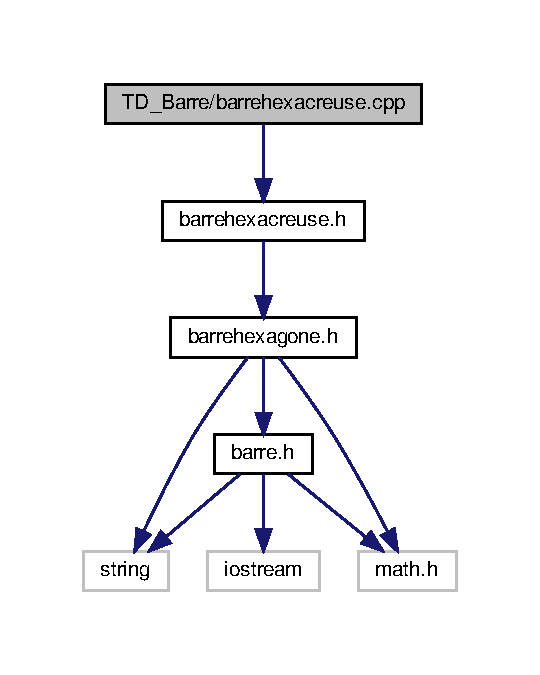
\includegraphics[width=259pt]{barrehexacreuse_8cpp__incl}
\end{center}
\end{figure}
